\documentclass[12pt,ngerman,parskip=half]{scrartcl}

\usepackage[utf8]{inputenc}
\usepackage[T1]{fontenc}
\usepackage{booktabs}
\usepackage{babel}
\usepackage{graphicx}
\usepackage{csquotes}
\usepackage{paralist}
\usepackage{xcolor}
\usepackage[]{blindtext}

\usepackage{tikz}

\begin{document}

\blindtext

\begin{figure}[h]
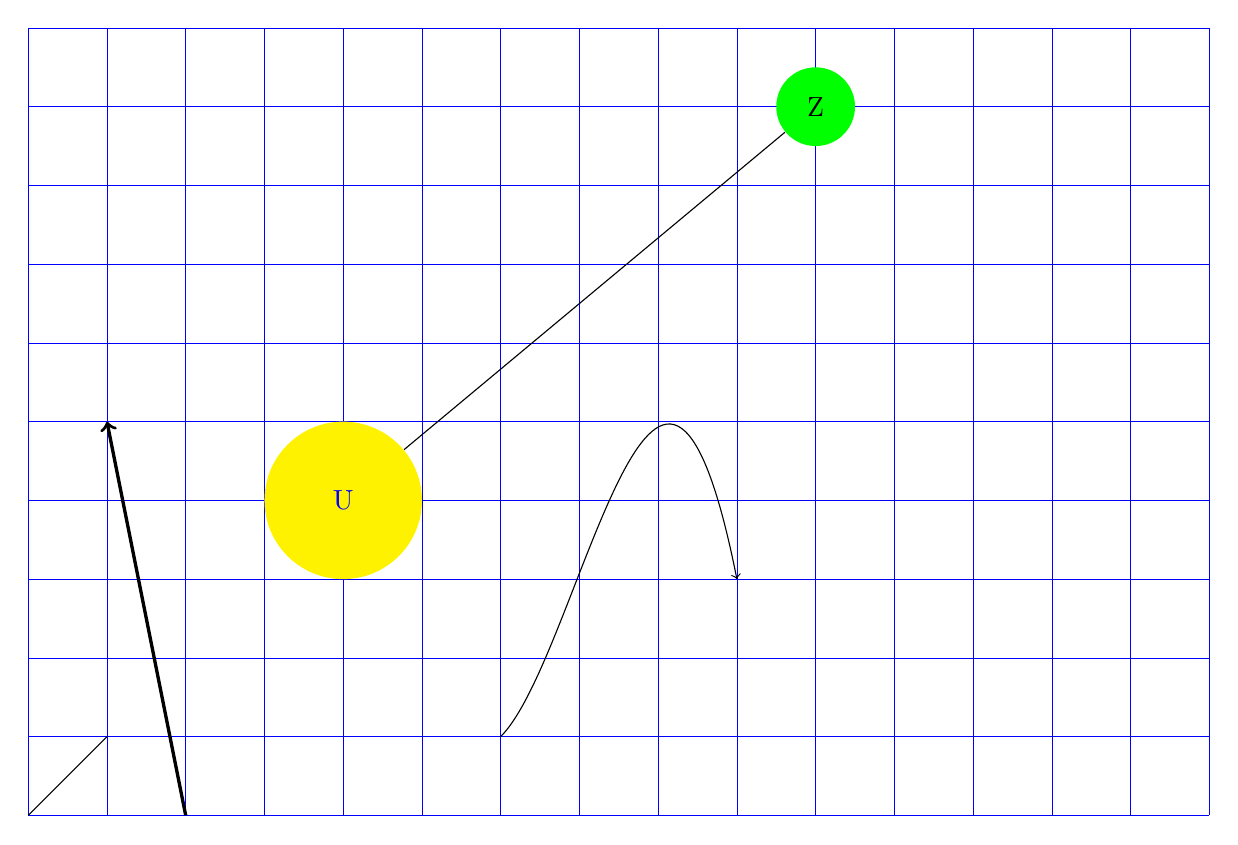
\begin{tikzpicture}[
punkt/.style={circle, minimum size = 2cm, blue, fill=yellow},
kleinpunkt/.style={punkt, minimum size = 1cm, black, fill=green},
]
\draw[help lines,blue] (0,0) grid (15,10);

\draw (0,0) -- (1,1);

\draw[->,very thick] (2,0) -- (1,5);

\draw[->] (6,1) .. controls (7,2) and (8,8) .. (9,3);

\node[punkt] (A) at (4,4){U};
\node[kleinpunkt] (B) at (10,9){Z};

\draw (A) -- (B);

\end{tikzpicture}
\caption{Mein Bild}
\end{figure}

\blindtext

\end{document}